\documentclass[letterpaper,12pt]{article}
\usepackage[utf8]{inputenc}
\usepackage{fullpage}
\usepackage{courier}
\usepackage[margin=0.75in]{geometry}
\usepackage{listings}
\usepackage{color}
\usepackage{graphicx}
\usepackage[width=5in]{caption}
\usepackage{hyphenat}
\usepackage[section]{placeins}
\usepackage{cmll}
\usepackage{float}
\usepackage{hyperref}

% Format a sectionless paragraph
\newcommand*\unparagraph{
	\par
	\nopagebreak
	\vskip3.25ex plus1ex minus.2ex
	\noindent
}

% define extra colors
\definecolor{dkgreen}{rgb}{0,0.6,0}
\definecolor{purple}{RGB}{159,0,197}

% define the code listing format
\lstset{
	language=Python,
	basicstyle=\footnotesize\ttfamily,
	backgroundcolor=\color{white},
	showspaces=false,
	showstringspaces=false,
	frame=none,
	tabsize=3,
	keywordstyle=\color{purple},
	commentstyle=\color{dkgreen},
	stringstyle=\color{blue},
	escapeinside={\%*}{*)}
}

% define the title/header
\title{\Large CS 1428 Honors\\Lab 11}
\author{Jared Wallace}
\date{}

\begin{document}

\maketitle

\vspace{30mm}

\section*{Overview}
Today we will be entering the wild world of Python. Python is very different from
C++. One of the main differences is that Python is not compiled, but rather interpreted. Another
big difference is that Python uses whitespace instead of curly braces.

A brief listing of pros and cons of Python are below.
\begin{itemize}
    \item The interpreter allows instant testing
    \item Focus on problem solving, not details and syntax (for the most part)
    \item Code is very elegant looking
    \item Python is always slower than the equivalent C or C++ code
    \item It can be unclear why your program doesn't work sometimes, due to the nature of non static typing
\end{itemize}

Here's an example Python program that prints "Hello World"
\begin{lstlisting}
#!/usr/bin/python
print "Hello World"
\end{lstlisting}
That's all the code you need.

Python does not have "arrays" per se, but it does have \textbf{lists}. A list is simply a collection of things.
You can even have a list of lists if you really want. Getting the values out of a list is super easy as well.
For example, I'll create a list with the numbers 1-9 and print them out. To open the interpreter directly, just type
"python" into the terminal.
\begin{lstlisting}
>>>myList = [1,2,3,4,5,6,7,8,9]
>>>print myList
[1,2,3,4,5,6,7,8,9]
\end{lstlisting}

Well, what if we don't want the entire list at once? Python offers a very easy method for looping, called
for each. Remember, whitespace (spaces, tabs) matters in Python!
\begin{lstlisting}
>>>for element in myList:
... print element
...
1
2
3
4
5
6
7
8
9
\end{lstlisting}

Python also offers many different ways to manipulate the list, like reverse() and sort().

\section*{Program}
Alright, we are going to be creating a webpage today (don't worry, I'll give you the HTML part)
that aggregates RSS feeds and displays them upon page load. We will be using an API, or Application
Programming Interface, located at the following address: \url{https://wiki.python.org/moin/RssLibraries}.

I have provided the skeleton code, but you will need to read the API page to figure out how to implement
the feed display. It's highly recommended you utilize the interpreter for debugging.


\section*{Grading}
Your implementation of this program is worth 100 points. For an extra 10 bonus points,
you may implement a binary search method in place of the default selection sort (rename your function in this case)


\section*{Deliverables}
Hard copy of the source code you wrote (happy.cpp). Soft copy (upload to homework upload) of
your source code. You may, at your discretion, use Git for version control -- it is not required.

% Comic at the bottom
%\begin{figure}[ht!]
%\centering
%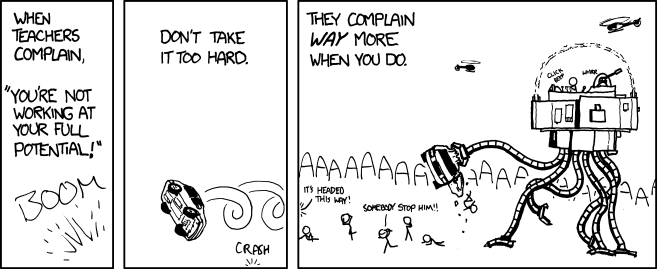
\includegraphics[width=6in]{potential.png}
%\caption*{The bunch of disadvantaged kids I was tutoring became too good at writing, and their essays were forcing me to confront painful existential questions, so I started trying to turn them on to drugs and crime instead.}
%\end{figure}
\end{document}
